É suficiente provar que $2\ell^2 \le S \le \frac{1}{2} L^2$.

\begin{lem*}
	$ 2\ell^2 \le S $
\end{lem*}

\begin{figure}[h]
	\begin{center}
		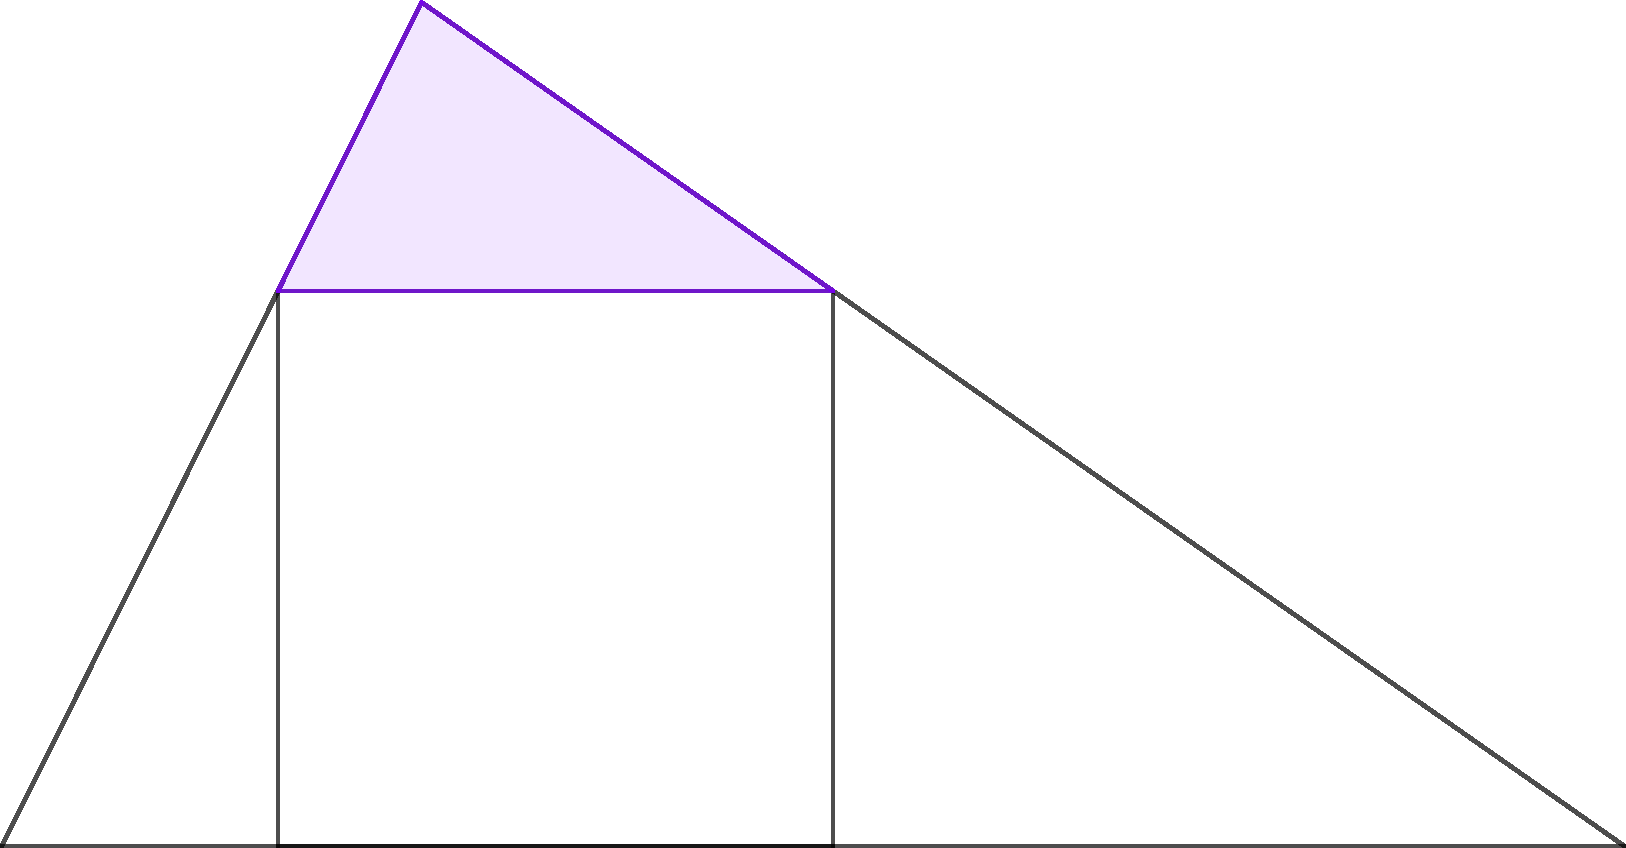
\includegraphics[width = 0.3\textwidth]{diagram_4}
		\caption{Diagrama auxiliar}
	\end{center}
\end{figure}

\begin{dem*}
	Note que o triângulo roxo é semelhante ao triângulo maior. Dessa forma, a razão da altura e da base, temos:
	\begin{gather*}
		\frac{h_a}{a} = \frac{h_a - \ell}{\ell}\\
		\ell = \frac{1}{\frac{1}{h_a} + \frac{1}{a}}
	\end{gather*}

	Portanto, $2\ell$ é a média harmônica entre $h_a$ e $a$, que é menor ou igual a média geométrica entre $h_a$ e $a$, e então:
	\begin{gather*}
		2\ell \le \sqrt{h_a a} = \sqrt{2S} \\
		2\ell^2 \le S
	\end{gather*}

	Com igualdade se, e somente se $h_a = a$
\end{dem*}

\begin{lem*}
	$ S \le \frac{1}{2} L^2 $
\end{lem*}

\begin{dem*}
	\begin{equation*}
		S =
		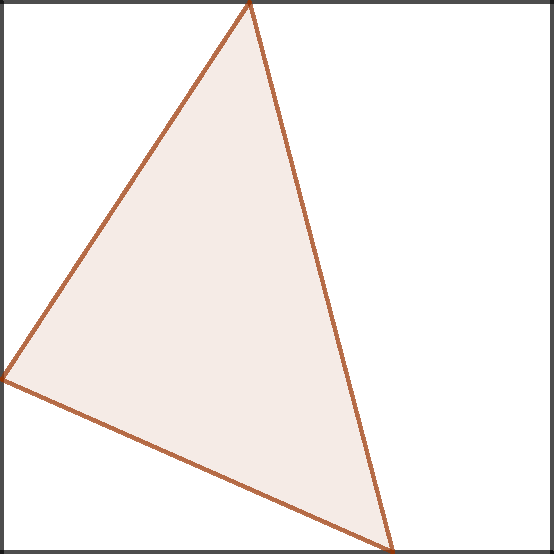
\includegraphics[align = c, width = 0.1\textwidth]{diagram_1}
		\le
		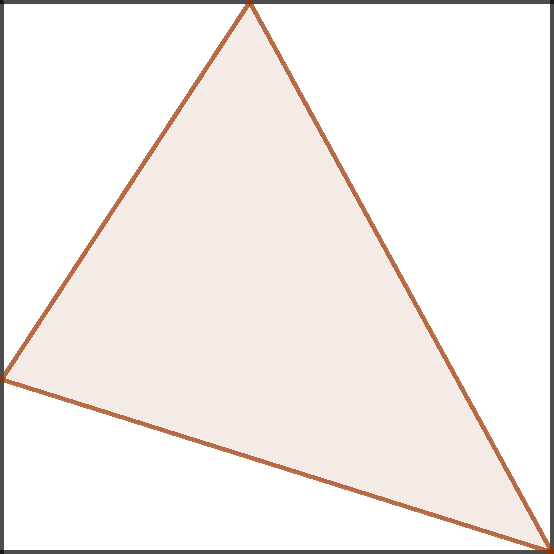
\includegraphics[align = c, width = 0.1\textwidth]{diagram_2}
		\le
		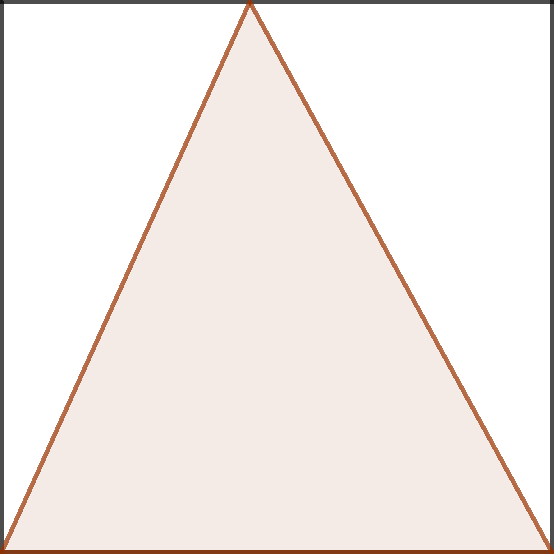
\includegraphics[align = c, width = 0.1\textwidth]{diagram_3}
		=
		\frac{1}{2} L^2
	\end{equation*}

	Com igualdade se, e somente se, dois vértices estão no quadrado $\iff$ alguma das bases do triângulo é igual à altura relativa.
\end{dem*}
